\documentclass[1p]{elsarticle_modified}
%\bibliographystyle{elsarticle-num}

%\usepackage[colorlinks]{hyperref}
%\usepackage{abbrmath_seonhwa} %\Abb, \Ascr, \Acal ,\Abf, \Afrak
\usepackage{amsfonts}
\usepackage{amssymb}
\usepackage{amsmath}
\usepackage{amsthm}
\usepackage{scalefnt}
\usepackage{amsbsy}
\usepackage{kotex}
\usepackage{caption}
\usepackage{subfig}
\usepackage{color}
\usepackage{graphicx}
\usepackage{xcolor} %% white, black, red, green, blue, cyan, magenta, yellow
\usepackage{float}
\usepackage{setspace}
\usepackage{hyperref}

\usepackage{tikz}
\usetikzlibrary{arrows}

\usepackage{multirow}
\usepackage{array} % fixed length table
\usepackage{hhline}

%%%%%%%%%%%%%%%%%%%%%
\makeatletter
\renewcommand*\env@matrix[1][\arraystretch]{%
	\edef\arraystretch{#1}%
	\hskip -\arraycolsep
	\let\@ifnextchar\new@ifnextchar
	\array{*\c@MaxMatrixCols c}}
\makeatother %https://tex.stackexchange.com/questions/14071/how-can-i-increase-the-line-spacing-in-a-matrix
%%%%%%%%%%%%%%%

\usepackage[normalem]{ulem}

\newcommand{\msout}[1]{\ifmmode\text{\sout{\ensuremath{#1}}}\else\sout{#1}\fi}
%SOURCE: \msout is \stkout macro in https://tex.stackexchange.com/questions/20609/strikeout-in-math-mode

\newcommand{\cancel}[1]{
	\ifmmode
	{\color{red}\msout{#1}}
	\else
	{\color{red}\sout{#1}}
	\fi
}

\newcommand{\add}[1]{
	{\color{blue}\uwave{#1}}
}

\newcommand{\replace}[2]{
	\ifmmode
	{\color{red}\msout{#1}}{\color{blue}\uwave{#2}}
	\else
	{\color{red}\sout{#1}}{\color{blue}\uwave{#2}}
	\fi
}

\newcommand{\Sol}{\mathcal{S}} %segment
\newcommand{\D}{D} %diagram
\newcommand{\A}{\mathcal{A}} %arc


%%%%%%%%%%%%%%%%%%%%%%%%%%%%%5 test

\def\sl{\operatorname{\textup{SL}}(2,\Cbb)}
\def\psl{\operatorname{\textup{PSL}}(2,\Cbb)}
\def\quan{\mkern 1mu \triangleright \mkern 1mu}

\theoremstyle{definition}
\newtheorem{thm}{Theorem}[section]
\newtheorem{prop}[thm]{Proposition}
\newtheorem{lem}[thm]{Lemma}
\newtheorem{ques}[thm]{Question}
\newtheorem{cor}[thm]{Corollary}
\newtheorem{defn}[thm]{Definition}
\newtheorem{exam}[thm]{Example}
\newtheorem{rmk}[thm]{Remark}
\newtheorem{alg}[thm]{Algorithm}

\newcommand{\I}{\sqrt{-1}}
\begin{document}

%\begin{frontmatter}
%
%\title{Boundary parabolic representations of knots up to 8 crossings}
%
%%% Group authors per affiliation:
%\author{Yunhi Cho} 
%\address{Department of Mathematics, University of Seoul, Seoul, Korea}
%\ead{yhcho@uos.ac.kr}
%
%
%\author{Seonhwa Kim} %\fnref{s_kim}}
%\address{Center for Geometry and Physics, Institute for Basic Science, Pohang, 37673, Korea}
%\ead{ryeona17@ibs.re.kr}
%
%\author{Hyuk Kim}
%\address{Department of Mathematical Sciences, Seoul National University, Seoul 08826, Korea}
%\ead{hyukkim@snu.ac.kr}
%
%\author{Seokbeom Yoon}
%\address{Department of Mathematical Sciences, Seoul National University, Seoul, 08826,  Korea}
%\ead{sbyoon15@snu.ac.kr}
%
%\begin{abstract}
%We find all boundary parabolic representation of knots up to 8 crossings.
%
%\end{abstract}
%\begin{keyword}
%    \MSC[2010] 57M25 
%\end{keyword}
%
%\end{frontmatter}

%\linenumbers
%\tableofcontents
%
\newcommand\colored[1]{\textcolor{white}{\rule[-0.35ex]{0.8em}{1.4ex}}\kern-0.8em\color{red} #1}%
%\newcommand\colored[1]{\textcolor{white}{ #1}\kern-2.17ex	\textcolor{white}{ #1}\kern-1.81ex	\textcolor{white}{ #1}\kern-2.15ex\color{red}#1	}

{\Large $\underline{12n_{0811}~(K12n_{0811})}$}

\setlength{\tabcolsep}{10pt}
\renewcommand{\arraystretch}{1.6}
\vspace{1cm}\begin{tabular}{m{100pt}>{\centering\arraybackslash}m{274pt}}
\multirow{5}{120pt}{
	\centering
	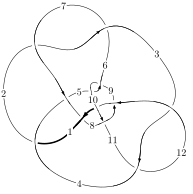
\includegraphics[width=112pt]{../../../GIT/diagram.site/Diagrams/png/2900_12n_0811.png}\\
\ \ \ A knot diagram\footnotemark}&
\allowdisplaybreaks
\textbf{Linearized knot diagam} \\
\cline{2-2}
 &
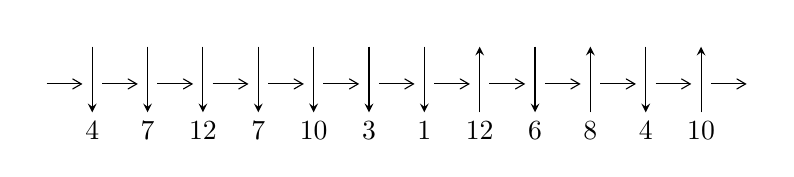
\begin{tikzpicture}[x=20pt, y=17pt]
	% nodes
	\node (C0) at (0, 0) {};
	\node (C1) at (1, 0) {};
	\node (C1U) at (1, +1) {};
	\node (C1D) at (1, -1) {4};

	\node (C2) at (2, 0) {};
	\node (C2U) at (2, +1) {};
	\node (C2D) at (2, -1) {7};

	\node (C3) at (3, 0) {};
	\node (C3U) at (3, +1) {};
	\node (C3D) at (3, -1) {12};

	\node (C4) at (4, 0) {};
	\node (C4U) at (4, +1) {};
	\node (C4D) at (4, -1) {7};

	\node (C5) at (5, 0) {};
	\node (C5U) at (5, +1) {};
	\node (C5D) at (5, -1) {10};

	\node (C6) at (6, 0) {};
	\node (C6U) at (6, +1) {};
	\node (C6D) at (6, -1) {3};

	\node (C7) at (7, 0) {};
	\node (C7U) at (7, +1) {};
	\node (C7D) at (7, -1) {1};

	\node (C8) at (8, 0) {};
	\node (C8U) at (8, +1) {};
	\node (C8D) at (8, -1) {12};

	\node (C9) at (9, 0) {};
	\node (C9U) at (9, +1) {};
	\node (C9D) at (9, -1) {6};

	\node (C10) at (10, 0) {};
	\node (C10U) at (10, +1) {};
	\node (C10D) at (10, -1) {8};

	\node (C11) at (11, 0) {};
	\node (C11U) at (11, +1) {};
	\node (C11D) at (11, -1) {4};

	\node (C12) at (12, 0) {};
	\node (C12U) at (12, +1) {};
	\node (C12D) at (12, -1) {10};
	\node (C13) at (13, 0) {};

	% arrows
	\draw[->,>={angle 60}]
	(C0) edge (C1) (C1) edge (C2) (C2) edge (C3) (C3) edge (C4) (C4) edge (C5) (C5) edge (C6) (C6) edge (C7) (C7) edge (C8) (C8) edge (C9) (C9) edge (C10) (C10) edge (C11) (C11) edge (C12) (C12) edge (C13) ;	\draw[->,>=stealth]
	(C1U) edge (C1D) (C2U) edge (C2D) (C3U) edge (C3D) (C4U) edge (C4D) (C5U) edge (C5D) (C6U) edge (C6D) (C7U) edge (C7D) (C8D) edge (C8U) (C9U) edge (C9D) (C10D) edge (C10U) (C11U) edge (C11D) (C12D) edge (C12U) ;
	\end{tikzpicture} \\
\hhline{~~} \\& 
\textbf{Solving Sequence} \\ \cline{2-2} 
 &
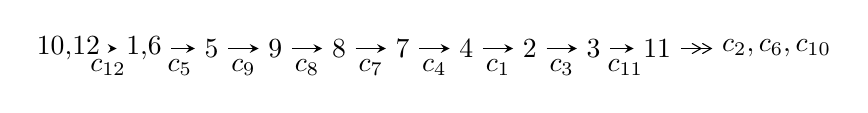
\begin{tikzpicture}[x=23pt, y=7pt]
	% node
	\node (A0) at (-1/8, 0) {10,12};
	\node (A1) at (17/16, 0) {1,6};
	\node (A2) at (17/8, 0) {5};
	\node (A3) at (25/8, 0) {9};
	\node (A4) at (33/8, 0) {8};
	\node (A5) at (41/8, 0) {7};
	\node (A6) at (49/8, 0) {4};
	\node (A7) at (57/8, 0) {2};
	\node (A8) at (65/8, 0) {3};
	\node (A9) at (73/8, 0) {11};
	\node (C1) at (1/2, -1) {$c_{12}$};
	\node (C2) at (13/8, -1) {$c_{5}$};
	\node (C3) at (21/8, -1) {$c_{9}$};
	\node (C4) at (29/8, -1) {$c_{8}$};
	\node (C5) at (37/8, -1) {$c_{7}$};
	\node (C6) at (45/8, -1) {$c_{4}$};
	\node (C7) at (53/8, -1) {$c_{1}$};
	\node (C8) at (61/8, -1) {$c_{3}$};
	\node (C9) at (69/8, -1) {$c_{11}$};
	\node (A10) at (11, 0) {$c_{2},c_{6},c_{10}$};

	% edge
	\draw[->,>=stealth]	
	(A0) edge (A1) (A1) edge (A2) (A2) edge (A3) (A3) edge (A4) (A4) edge (A5) (A5) edge (A6) (A6) edge (A7) (A7) edge (A8) (A8) edge (A9) ;
	\draw[->>,>={angle 60}]	
	(A9) edge (A10);
\end{tikzpicture} \\ 

\end{tabular} \\

\footnotetext{
The image of knot diagram is generated by the software ``\textbf{Draw programme}" developed by Andrew Bartholomew(\url{http://www.layer8.co.uk/maths/draw/index.htm\#Running-draw}), where we modified some parts for our purpose(\url{https://github.com/CATsTAILs/LinksPainter}).
}\phantom \\ \newline 
\centering \textbf{Ideals for irreducible components\footnotemark of $X_{\text{par}}$} 
 
\begin{align*}
I^u_{1}&=\langle 
-238 u^{15}+537 u^{14}+\cdots+1291 b+644,\;-932 u^{15}-273 u^{14}+\cdots+1291 a+3661,\\
\phantom{I^u_{1}}&\phantom{= \langle  }u^{16}-4 u^{14}+4 u^{13}+12 u^{12}-18 u^{11}-13 u^{10}+44 u^9-6 u^8-55 u^7+38 u^6+30 u^5-42 u^4+u^3+17 u^2-6 u-1\rangle \\
I^u_{2}&=\langle 
1.11360\times10^{68} u^{37}-1.13094\times10^{68} u^{36}+\cdots+3.45683\times10^{69} b-5.20337\times10^{69},\\
\phantom{I^u_{2}}&\phantom{= \langle  }-1.43917\times10^{70} u^{37}+2.46784\times10^{70} u^{36}+\cdots+2.73089\times10^{71} a+1.06137\times10^{72},\\
\phantom{I^u_{2}}&\phantom{= \langle  }u^{38}- u^{37}+\cdots-62 u-79\rangle \\
I^u_{3}&=\langle 
23118092 u^{15}-125359960 u^{14}+\cdots+12462493 b-54569021,\\
\phantom{I^u_{3}}&\phantom{= \langle  }21062121 u^{15}-121014315 u^{14}+\cdots+12462493 a-38321689,\;u^{16}-6 u^{15}+\cdots-4 u+1\rangle \\
I^u_{4}&=\langle 
- u^5+u^3-2 u^2+b- u+1,\;- u^5+2 u^3-2 u^2+a-2 u+2,\;u^6+u^5-2 u^4+3 u^2- u-1\rangle \\
I^u_{5}&=\langle 
b-1,\;a,\;u-1\rangle \\
\\
\end{align*}
\raggedright * 5 irreducible components of $\dim_{\mathbb{C}}=0$, with total 77 representations.\\
\footnotetext{All coefficients of polynomials are rational numbers. But the coefficients are sometimes approximated in decimal forms when there is not enough margin.}
\newpage
\renewcommand{\arraystretch}{1}
\centering \section*{I. $I^u_{1}= \langle -238 u^{15}+537 u^{14}+\cdots+1291 b+644,\;-932 u^{15}-273 u^{14}+\cdots+1291 a+3661,\;u^{16}-4 u^{14}+\cdots-6 u-1 \rangle$}
\flushleft \textbf{(i) Arc colorings}\\
\begin{tabular}{m{7pt} m{180pt} m{7pt} m{180pt} }
\flushright $a_{10}=$&$\begin{pmatrix}0\\u\end{pmatrix}$ \\
\flushright $a_{12}=$&$\begin{pmatrix}1\\0\end{pmatrix}$ \\
\flushright $a_{1}=$&$\begin{pmatrix}1\\- u^2\end{pmatrix}$ \\
\flushright $a_{6}=$&$\begin{pmatrix}0.721921 u^{15}+0.211464 u^{14}+\cdots+4.89388 u-2.83579\\0.184353 u^{15}-0.415957 u^{14}+\cdots+1.94500 u-0.498838\end{pmatrix}$ \\
\flushright $a_{5}=$&$\begin{pmatrix}0.721921 u^{15}+0.211464 u^{14}+\cdots+4.89388 u-2.83579\\-0.367932 u^{15}-0.711851 u^{14}+\cdots-0.0457010 u-0.710302\end{pmatrix}$ \\
\flushright $a_{9}=$&$\begin{pmatrix}-0.0503486 u^{15}+0.344694 u^{14}+\cdots+3.12006 u-0.981410\\-0.0503486 u^{15}+0.344694 u^{14}+\cdots+3.12006 u+0.0185902\end{pmatrix}$ \\
\flushright $a_{8}=$&$\begin{pmatrix}-1\\-0.0503486 u^{15}+0.344694 u^{14}+\cdots+3.12006 u+0.0185902\end{pmatrix}$ \\
\flushright $a_{7}=$&$\begin{pmatrix}-0.0503486 u^{15}+0.344694 u^{14}+\cdots+3.12006 u-0.981410\\-0.0751356 u^{15}-0.254841 u^{14}+\cdots+1.10225 u-0.326104\end{pmatrix}$ \\
\flushright $a_{4}=$&$\begin{pmatrix}0.537568 u^{15}+0.627421 u^{14}+\cdots+2.94888 u-2.33695\\-0.211464 u^{15}-0.552285 u^{14}+\cdots-1.49574 u-0.721921\end{pmatrix}$ \\
\flushright $a_{2}=$&$\begin{pmatrix}-0.333075 u^{15}-0.181255 u^{14}+\cdots+0.948102 u+2.43067\\0.344694 u^{15}+0.0247870 u^{14}+\cdots-1.28350 u-0.0503486\end{pmatrix}$ \\
\flushright $a_{3}=$&$\begin{pmatrix}0.326104 u^{15}+0.0751356 u^{14}+\cdots+1.45314 u-3.05887\\-0.211464 u^{15}-0.552285 u^{14}+\cdots-1.49574 u-0.721921\end{pmatrix}$ \\
\flushright $a_{11}=$&$\begin{pmatrix}u\\-0.344694 u^{15}-0.0247870 u^{14}+\cdots+1.28350 u+0.0503486\end{pmatrix}$\\&\end{tabular}
\flushleft \textbf{(ii) Obstruction class $= -1$}\\~\\
\flushleft \textbf{(iii) Cusp Shapes $= \frac{4859}{1291} u^{15}-\frac{196}{1291} u^{14}+\cdots+\frac{57432}{1291} u-\frac{9123}{1291}$}\\~\\
\newpage\renewcommand{\arraystretch}{1}
\flushleft \textbf{(iv) u-Polynomials at the component}\newline \\
\begin{tabular}{m{50pt}|m{274pt}}
Crossings & \hspace{64pt}u-Polynomials at each crossing \\
\hline $$\begin{aligned}c_{1},c_{4}\end{aligned}$$&$\begin{aligned}
&u^{16}- u^{15}+\cdots-8 u+1
\end{aligned}$\\
\hline $$\begin{aligned}c_{2},c_{6}\end{aligned}$$&$\begin{aligned}
&u^{16}+8 u^{15}+\cdots+20 u-8
\end{aligned}$\\
\hline $$\begin{aligned}c_{3},c_{5},c_{9}\\c_{11}\end{aligned}$$&$\begin{aligned}
&u^{16}+u^{15}+\cdots+8 u+2
\end{aligned}$\\
\hline $$\begin{aligned}c_{7}\end{aligned}$$&$\begin{aligned}
&u^{16}-15 u^{15}+\cdots+384 u-64
\end{aligned}$\\
\hline $$\begin{aligned}c_{8}\end{aligned}$$&$\begin{aligned}
&u^{16}-23 u^{15}+\cdots+2952 u-472
\end{aligned}$\\
\hline $$\begin{aligned}c_{10},c_{12}\end{aligned}$$&$\begin{aligned}
&u^{16}-4 u^{14}+\cdots-6 u-1
\end{aligned}$\\
\hline
\end{tabular}\\~\\
\newpage\renewcommand{\arraystretch}{1}
\flushleft \textbf{(v) Riley Polynomials at the component}\newline \\
\begin{tabular}{m{50pt}|m{274pt}}
Crossings & \hspace{64pt}Riley Polynomials at each crossing \\
\hline $$\begin{aligned}c_{1},c_{4}\end{aligned}$$&$\begin{aligned}
&y^{16}-23 y^{15}+\cdots-32 y+1
\end{aligned}$\\
\hline $$\begin{aligned}c_{2},c_{6}\end{aligned}$$&$\begin{aligned}
&y^{16}+8 y^{15}+\cdots-1232 y+64
\end{aligned}$\\
\hline $$\begin{aligned}c_{3},c_{5},c_{9}\\c_{11}\end{aligned}$$&$\begin{aligned}
&y^{16}+13 y^{15}+\cdots+16 y+4
\end{aligned}$\\
\hline $$\begin{aligned}c_{7}\end{aligned}$$&$\begin{aligned}
&y^{16}- y^{15}+\cdots-30720 y+4096
\end{aligned}$\\
\hline $$\begin{aligned}c_{8}\end{aligned}$$&$\begin{aligned}
&y^{16}-31 y^{15}+\cdots-1605984 y+222784
\end{aligned}$\\
\hline $$\begin{aligned}c_{10},c_{12}\end{aligned}$$&$\begin{aligned}
&y^{16}-8 y^{15}+\cdots-70 y+1
\end{aligned}$\\
\hline
\end{tabular}\\~\\
\newpage\flushleft \textbf{(vi) Complex Volumes and Cusp Shapes}
$$\begin{array}{c|c|c}  
\text{Solutions to }I^u_{1}& \I (\text{vol} + \sqrt{-1}CS) & \text{Cusp shape}\\
 \hline 
\begin{aligned}
u &= \phantom{-}0.728978 + 0.677201 I \\
a &= \phantom{-}0.532336 + 0.060278 I \\
b &= -0.100353 - 1.153050 I\end{aligned}
 & -2.58048 + 3.00554 I & -8.10520 - 2.38597 I \\ \hline\begin{aligned}
u &= \phantom{-}0.728978 - 0.677201 I \\
a &= \phantom{-}0.532336 - 0.060278 I \\
b &= -0.100353 + 1.153050 I\end{aligned}
 & -2.58048 - 3.00554 I & -8.10520 + 2.38597 I \\ \hline\begin{aligned}
u &= -0.973288 + 0.184794 I \\
a &= \phantom{-}0.75785 + 1.37831 I \\
b &= \phantom{-}0.04286 + 2.43021 I\end{aligned}
 & \phantom{-}8.11198 - 4.38794 I & -0.64562 + 2.92845 I \\ \hline\begin{aligned}
u &= -0.973288 - 0.184794 I \\
a &= \phantom{-}0.75785 - 1.37831 I \\
b &= \phantom{-}0.04286 - 2.43021 I\end{aligned}
 & \phantom{-}8.11198 + 4.38794 I & -0.64562 - 2.92845 I \\ \hline\begin{aligned}
u &= \phantom{-}0.888929\phantom{ +0.000000I} \\
a &= \phantom{-}1.47043\phantom{ +0.000000I} \\
b &= \phantom{-}1.55541\phantom{ +0.000000I}\end{aligned}
 & -3.37262\phantom{ +0.000000I} & -0.442120\phantom{ +0.000000I} \\ \hline\begin{aligned}
u &= \phantom{-}0.758242 + 0.439908 I \\
a &= -0.459222 - 0.501064 I \\
b &= \phantom{-}0.174916 + 0.053608 I\end{aligned}
 & \phantom{-}1.34319 + 1.06797 I & \phantom{-}1.49479 - 2.77265 I \\ \hline\begin{aligned}
u &= \phantom{-}0.758242 - 0.439908 I \\
a &= -0.459222 + 0.501064 I \\
b &= \phantom{-}0.174916 - 0.053608 I\end{aligned}
 & \phantom{-}1.34319 - 1.06797 I & \phantom{-}1.49479 + 2.77265 I \\ \hline\begin{aligned}
u &= -1.184440 + 0.400458 I \\
a &= -0.342142 + 1.050790 I \\
b &= -0.07013 + 2.63493 I\end{aligned}
 & \phantom{-}1.19975 - 5.05833 I & -0.62604 + 3.74336 I \\ \hline\begin{aligned}
u &= -1.184440 - 0.400458 I \\
a &= -0.342142 - 1.050790 I \\
b &= -0.07013 - 2.63493 I\end{aligned}
 & \phantom{-}1.19975 + 5.05833 I & -0.62604 - 3.74336 I \\ \hline\begin{aligned}
u &= \phantom{-}0.939130 + 0.905743 I \\
a &= \phantom{-}0.479797 + 0.632021 I \\
b &= -0.395886 + 0.676605 I\end{aligned}
 & \phantom{-}6.57781 + 4.06178 I & \phantom{-}0.252631 - 0.871494 I\\
 \hline 
 \end{array}$$\newpage$$\begin{array}{c|c|c}  
\text{Solutions to }I^u_{1}& \I (\text{vol} + \sqrt{-1}CS) & \text{Cusp shape}\\
 \hline 
\begin{aligned}
u &= \phantom{-}0.939130 - 0.905743 I \\
a &= \phantom{-}0.479797 - 0.632021 I \\
b &= -0.395886 - 0.676605 I\end{aligned}
 & \phantom{-}6.57781 - 4.06178 I & \phantom{-}0.252631 + 0.871494 I \\ \hline\begin{aligned}
u &= \phantom{-}0.778111 + 1.047600 I \\
a &= -1.027370 - 0.416604 I \\
b &= -0.364894 - 0.086454 I\end{aligned}
 & \phantom{-}1.69590 - 0.28714 I & -3.98649 + 0.31929 I \\ \hline\begin{aligned}
u &= \phantom{-}0.778111 - 1.047600 I \\
a &= -1.027370 + 0.416604 I \\
b &= -0.364894 + 0.086454 I\end{aligned}
 & \phantom{-}1.69590 + 0.28714 I & -3.98649 - 0.31929 I \\ \hline\begin{aligned}
u &= -1.42884 + 0.78989 I \\
a &= -0.004460 - 1.145420 I \\
b &= \phantom{-}0.25947 - 2.48543 I\end{aligned}
 & \phantom{-}6.3323 - 15.0071 I & -2.77467 + 7.02006 I \\ \hline\begin{aligned}
u &= -1.42884 - 0.78989 I \\
a &= -0.004460 + 1.145420 I \\
b &= \phantom{-}0.25947 + 2.48543 I\end{aligned}
 & \phantom{-}6.3323 + 15.0071 I & -2.77467 - 7.02006 I \\ \hline\begin{aligned}
u &= -0.124728\phantom{ +0.000000I} \\
a &= -3.34399\phantom{ +0.000000I} \\
b &= -0.647391\phantom{ +0.000000I}\end{aligned}
 & -0.864939\phantom{ +0.000000I} & -12.7770\phantom{ +0.000000I}\\
 \hline 
 \end{array}$$\newpage\newpage\renewcommand{\arraystretch}{1}
\centering \section*{II. $I^u_{2}= \langle 1.11\times10^{68} u^{37}-1.13\times10^{68} u^{36}+\cdots+3.46\times10^{69} b-5.20\times10^{69},\;-1.44\times10^{70} u^{37}+2.47\times10^{70} u^{36}+\cdots+2.73\times10^{71} a+1.06\times10^{72},\;u^{38}- u^{37}+\cdots-62 u-79 \rangle$}
\flushleft \textbf{(i) Arc colorings}\\
\begin{tabular}{m{7pt} m{180pt} m{7pt} m{180pt} }
\flushright $a_{10}=$&$\begin{pmatrix}0\\u\end{pmatrix}$ \\
\flushright $a_{12}=$&$\begin{pmatrix}1\\0\end{pmatrix}$ \\
\flushright $a_{1}=$&$\begin{pmatrix}1\\- u^2\end{pmatrix}$ \\
\flushright $a_{6}=$&$\begin{pmatrix}0.0526998 u^{37}-0.0903674 u^{36}+\cdots+6.01858 u-3.88653\\-0.0322146 u^{37}+0.0327163 u^{36}+\cdots-13.6241 u+1.50524\end{pmatrix}$ \\
\flushright $a_{5}=$&$\begin{pmatrix}0.0526998 u^{37}-0.0903674 u^{36}+\cdots+6.01858 u-3.88653\\-0.0656788 u^{37}+0.0946351 u^{36}+\cdots-15.4520 u+4.48099\end{pmatrix}$ \\
\flushright $a_{9}=$&$\begin{pmatrix}-0.0923222 u^{37}+0.172239 u^{36}+\cdots-2.83315 u+10.5939\\-0.0552169 u^{37}+0.106775 u^{36}+\cdots-3.51727 u+1.07664\end{pmatrix}$ \\
\flushright $a_{8}=$&$\begin{pmatrix}-0.0371054 u^{37}+0.0654636 u^{36}+\cdots+0.684120 u+9.51724\\-0.0552169 u^{37}+0.106775 u^{36}+\cdots-3.51727 u+1.07664\end{pmatrix}$ \\
\flushright $a_{7}=$&$\begin{pmatrix}-0.109138 u^{37}+0.206389 u^{36}+\cdots-4.00626 u+12.8342\\0.0102538 u^{37}-0.0153113 u^{36}+\cdots-2.09807 u-4.36588\end{pmatrix}$ \\
\flushright $a_{4}=$&$\begin{pmatrix}-0.0615144 u^{37}+0.0746738 u^{36}+\cdots-6.24915 u+6.93837\\-0.0514669 u^{37}+0.116872 u^{36}+\cdots+4.44234 u+3.78722\end{pmatrix}$ \\
\flushright $a_{2}=$&$\begin{pmatrix}-0.0418893 u^{37}+0.0332093 u^{36}+\cdots-18.2103 u+7.21885\\-0.0520505 u^{37}+0.129376 u^{36}+\cdots+7.63964 u+3.43879\end{pmatrix}$ \\
\flushright $a_{3}=$&$\begin{pmatrix}-0.112981 u^{37}+0.191546 u^{36}+\cdots-1.80681 u+10.7256\\-0.0514669 u^{37}+0.116872 u^{36}+\cdots+4.44234 u+3.78722\end{pmatrix}$ \\
\flushright $a_{11}=$&$\begin{pmatrix}0.0830893 u^{37}-0.117168 u^{36}+\cdots+22.3030 u-10.8514\\0.0370786 u^{37}-0.0992755 u^{36}+\cdots-12.0908 u-0.746538\end{pmatrix}$\\&\end{tabular}
\flushleft \textbf{(ii) Obstruction class $= -1$}\\~\\
\flushleft \textbf{(iii) Cusp Shapes $= 0.0873374 u^{37}-0.323866 u^{36}+\cdots-73.1911 u-23.6929$}\\~\\
\newpage\renewcommand{\arraystretch}{1}
\flushleft \textbf{(iv) u-Polynomials at the component}\newline \\
\begin{tabular}{m{50pt}|m{274pt}}
Crossings & \hspace{64pt}u-Polynomials at each crossing \\
\hline $$\begin{aligned}c_{1},c_{4}\end{aligned}$$&$\begin{aligned}
&u^{38}-4 u^{37}+\cdots+2639 u-353
\end{aligned}$\\
\hline $$\begin{aligned}c_{2},c_{6}\end{aligned}$$&$\begin{aligned}
&(u^{19}-3 u^{18}+\cdots+65 u-25)^{2}
\end{aligned}$\\
\hline $$\begin{aligned}c_{3},c_{5},c_{9}\\c_{11}\end{aligned}$$&$\begin{aligned}
&u^{38}+11 u^{36}+\cdots+2730 u-2315
\end{aligned}$\\
\hline $$\begin{aligned}c_{7}\end{aligned}$$&$\begin{aligned}
&(u^{19}+6 u^{18}+\cdots+10 u+1)^{2}
\end{aligned}$\\
\hline $$\begin{aligned}c_{8}\end{aligned}$$&$\begin{aligned}
&(u^{19}+12 u^{18}+\cdots+1502 u+625)^{2}
\end{aligned}$\\
\hline $$\begin{aligned}c_{10},c_{12}\end{aligned}$$&$\begin{aligned}
&u^{38}- u^{37}+\cdots-62 u-79
\end{aligned}$\\
\hline
\end{tabular}\\~\\
\newpage\renewcommand{\arraystretch}{1}
\flushleft \textbf{(v) Riley Polynomials at the component}\newline \\
\begin{tabular}{m{50pt}|m{274pt}}
Crossings & \hspace{64pt}Riley Polynomials at each crossing \\
\hline $$\begin{aligned}c_{1},c_{4}\end{aligned}$$&$\begin{aligned}
&y^{38}-20 y^{37}+\cdots+770615 y+124609
\end{aligned}$\\
\hline $$\begin{aligned}c_{2},c_{6}\end{aligned}$$&$\begin{aligned}
&(y^{19}+17 y^{18}+\cdots-5175 y-625)^{2}
\end{aligned}$\\
\hline $$\begin{aligned}c_{3},c_{5},c_{9}\\c_{11}\end{aligned}$$&$\begin{aligned}
&y^{38}+22 y^{37}+\cdots+60589580 y+5359225
\end{aligned}$\\
\hline $$\begin{aligned}c_{7}\end{aligned}$$&$\begin{aligned}
&(y^{19}-12 y^{18}+\cdots+30 y-1)^{2}
\end{aligned}$\\
\hline $$\begin{aligned}c_{8}\end{aligned}$$&$\begin{aligned}
&(y^{19}-54 y^{18}+\cdots-2158996 y-390625)^{2}
\end{aligned}$\\
\hline $$\begin{aligned}c_{10},c_{12}\end{aligned}$$&$\begin{aligned}
&y^{38}-27 y^{37}+\cdots-169744 y+6241
\end{aligned}$\\
\hline
\end{tabular}\\~\\
\newpage\flushleft \textbf{(vi) Complex Volumes and Cusp Shapes}
$$\begin{array}{c|c|c}  
\text{Solutions to }I^u_{2}& \I (\text{vol} + \sqrt{-1}CS) & \text{Cusp shape}\\
 \hline 
\begin{aligned}
u &= -0.679846 + 0.698404 I \\
a &= -0.273776 + 0.556482 I \\
b &= -0.473737 + 0.789202 I\end{aligned}
 & -2.35949 + 0.16321 I & -2.70781 - 0.18622 I \\ \hline\begin{aligned}
u &= -0.679846 - 0.698404 I \\
a &= -0.273776 - 0.556482 I \\
b &= -0.473737 - 0.789202 I\end{aligned}
 & -2.35949 - 0.16321 I & -2.70781 + 0.18622 I \\ \hline\begin{aligned}
u &= \phantom{-}0.960122 + 0.435314 I \\
a &= \phantom{-}0.593065 - 0.764570 I \\
b &= -0.438163 - 1.282160 I\end{aligned}
 & -1.51388 + 1.79009 I & -4.72788 - 2.74496 I \\ \hline\begin{aligned}
u &= \phantom{-}0.960122 - 0.435314 I \\
a &= \phantom{-}0.593065 + 0.764570 I \\
b &= -0.438163 + 1.282160 I\end{aligned}
 & -1.51388 - 1.79009 I & -4.72788 + 2.74496 I \\ \hline\begin{aligned}
u &= -1.07632\phantom{ +0.000000I} \\
a &= \phantom{-}1.52827\phantom{ +0.000000I} \\
b &= \phantom{-}1.02377\phantom{ +0.000000I}\end{aligned}
 & -7.09286\phantom{ +0.000000I} & -34.9180\phantom{ +0.000000I} \\ \hline\begin{aligned}
u &= -0.189836 + 0.874146 I \\
a &= \phantom{-}0.036583 - 1.409850 I \\
b &= -0.274085 - 1.305950 I\end{aligned}
 & -2.35949 - 0.16321 I & -2.70781 + 0.18622 I \\ \hline\begin{aligned}
u &= -0.189836 - 0.874146 I \\
a &= \phantom{-}0.036583 + 1.409850 I \\
b &= -0.274085 + 1.305950 I\end{aligned}
 & -2.35949 + 0.16321 I & -2.70781 - 0.18622 I \\ \hline\begin{aligned}
u &= -0.879859 + 0.138648 I \\
a &= \phantom{-}1.18883 - 0.97573 I \\
b &= \phantom{-}0.737407 - 0.181415 I\end{aligned}
 & \phantom{-}7.75558 + 3.00592 I & -1.52759 - 2.83549 I \\ \hline\begin{aligned}
u &= -0.879859 - 0.138648 I \\
a &= \phantom{-}1.18883 + 0.97573 I \\
b &= \phantom{-}0.737407 + 0.181415 I\end{aligned}
 & \phantom{-}7.75558 - 3.00592 I & -1.52759 + 2.83549 I \\ \hline\begin{aligned}
u &= -1.058720 + 0.361703 I \\
a &= \phantom{-}0.182710 + 1.281260 I \\
b &= -0.60977 + 2.90746 I\end{aligned}
 & \phantom{-}10.82200 - 4.29446 I & -2.82455 + 4.66988 I\\
 \hline 
 \end{array}$$\newpage$$\begin{array}{c|c|c}  
\text{Solutions to }I^u_{2}& \I (\text{vol} + \sqrt{-1}CS) & \text{Cusp shape}\\
 \hline 
\begin{aligned}
u &= -1.058720 - 0.361703 I \\
a &= \phantom{-}0.182710 - 1.281260 I \\
b &= -0.60977 - 2.90746 I\end{aligned}
 & \phantom{-}10.82200 + 4.29446 I & -2.82455 - 4.66988 I \\ \hline\begin{aligned}
u &= -0.917174 + 0.653292 I \\
a &= \phantom{-}0.361519 - 0.436397 I \\
b &= \phantom{-}0.077422 + 0.149014 I\end{aligned}
 & -1.68798 - 5.37827 I & \phantom{-}0.03508 + 8.21916 I \\ \hline\begin{aligned}
u &= -0.917174 - 0.653292 I \\
a &= \phantom{-}0.361519 + 0.436397 I \\
b &= \phantom{-}0.077422 - 0.149014 I\end{aligned}
 & -1.68798 + 5.37827 I & \phantom{-}0.03508 - 8.21916 I \\ \hline\begin{aligned}
u &= \phantom{-}1.114930 + 0.331378 I \\
a &= -0.097416 - 1.249650 I \\
b &= -0.20466 - 2.97495 I\end{aligned}
 & \phantom{-}2.34940 + 5.26338 I & -1.37964 - 4.11831 I \\ \hline\begin{aligned}
u &= \phantom{-}1.114930 - 0.331378 I \\
a &= -0.097416 + 1.249650 I \\
b &= -0.20466 + 2.97495 I\end{aligned}
 & \phantom{-}2.34940 - 5.26338 I & -1.37964 + 4.11831 I \\ \hline\begin{aligned}
u &= -0.772346 + 0.321245 I \\
a &= \phantom{-}1.182060 - 0.764049 I \\
b &= \phantom{-}0.507053 + 0.918255 I\end{aligned}
 & \phantom{-}9.66886 + 1.37924 I & -3.48192 + 4.90124 I \\ \hline\begin{aligned}
u &= -0.772346 - 0.321245 I \\
a &= \phantom{-}1.182060 + 0.764049 I \\
b &= \phantom{-}0.507053 - 0.918255 I\end{aligned}
 & \phantom{-}9.66886 - 1.37924 I & -3.48192 - 4.90124 I \\ \hline\begin{aligned}
u &= \phantom{-}0.637865 + 0.264901 I \\
a &= \phantom{-}1.10480 + 1.21426 I \\
b &= -0.357558 - 0.149777 I\end{aligned}
 & \phantom{-}0.57050 - 2.67427 I & \phantom{-}0.072556 - 0.682395 I \\ \hline\begin{aligned}
u &= \phantom{-}0.637865 - 0.264901 I \\
a &= \phantom{-}1.10480 - 1.21426 I \\
b &= -0.357558 + 0.149777 I\end{aligned}
 & \phantom{-}0.57050 + 2.67427 I & \phantom{-}0.072556 + 0.682395 I \\ \hline\begin{aligned}
u &= \phantom{-}1.048900 + 0.822943 I \\
a &= \phantom{-}0.305122 + 0.894638 I \\
b &= \phantom{-}0.586337 + 1.200440 I\end{aligned}
 & \phantom{-}2.61541 + 7.05508 I & -3.99946 - 5.58788 I\\
 \hline 
 \end{array}$$\newpage$$\begin{array}{c|c|c}  
\text{Solutions to }I^u_{2}& \I (\text{vol} + \sqrt{-1}CS) & \text{Cusp shape}\\
 \hline 
\begin{aligned}
u &= \phantom{-}1.048900 - 0.822943 I \\
a &= \phantom{-}0.305122 - 0.894638 I \\
b &= \phantom{-}0.586337 - 1.200440 I\end{aligned}
 & \phantom{-}2.61541 - 7.05508 I & -3.99946 + 5.58788 I \\ \hline\begin{aligned}
u &= -0.407834 + 0.346492 I \\
a &= \phantom{-}1.26494 - 1.09438 I \\
b &= -1.010750 - 0.253529 I\end{aligned}
 & -1.51388 + 1.79009 I & -4.72788 - 2.74496 I \\ \hline\begin{aligned}
u &= -0.407834 - 0.346492 I \\
a &= \phantom{-}1.26494 + 1.09438 I \\
b &= -1.010750 + 0.253529 I\end{aligned}
 & -1.51388 - 1.79009 I & -4.72788 + 2.74496 I \\ \hline\begin{aligned}
u &= \phantom{-}1.27274 + 0.74326 I \\
a &= -0.483706 - 0.727031 I \\
b &= -0.12463 - 2.06088 I\end{aligned}
 & \phantom{-}7.75558 + 3.00592 I & -1.52759 - 2.83549 I \\ \hline\begin{aligned}
u &= \phantom{-}1.27274 - 0.74326 I \\
a &= -0.483706 + 0.727031 I \\
b &= -0.12463 + 2.06088 I\end{aligned}
 & \phantom{-}7.75558 - 3.00592 I & -1.52759 + 2.83549 I \\ \hline\begin{aligned}
u &= \phantom{-}0.87992 + 1.24235 I \\
a &= -0.116819 + 0.798464 I \\
b &= \phantom{-}0.65914 + 2.10587 I\end{aligned}
 & -1.68798 + 5.37827 I & \phantom{-0.000000 } 0. - 8.21916 I \\ \hline\begin{aligned}
u &= \phantom{-}0.87992 - 1.24235 I \\
a &= -0.116819 - 0.798464 I \\
b &= \phantom{-}0.65914 - 2.10587 I\end{aligned}
 & -1.68798 - 5.37827 I & \phantom{-0.000000 -}0. + 8.21916 I \\ \hline\begin{aligned}
u &= -0.25188 + 1.54807 I \\
a &= -1.122660 - 0.209177 I \\
b &= \phantom{-}0.206822 - 0.294680 I\end{aligned}
 & \phantom{-}2.61541 + 7.05508 I & -6.00000 - 5.58788 I \\ \hline\begin{aligned}
u &= -0.25188 - 1.54807 I \\
a &= -1.122660 + 0.209177 I \\
b &= \phantom{-}0.206822 + 0.294680 I\end{aligned}
 & \phantom{-}2.61541 - 7.05508 I & -6.00000 + 5.58788 I \\ \hline\begin{aligned}
u &= -1.52147 + 0.50416 I \\
a &= -1.238570 - 0.121447 I \\
b &= -0.791063 - 0.291030 I\end{aligned}
 & \phantom{-}2.34940 - 5.26338 I & \phantom{-0.000000 } 0\\
 \hline 
 \end{array}$$\newpage$$\begin{array}{c|c|c}  
\text{Solutions to }I^u_{2}& \I (\text{vol} + \sqrt{-1}CS) & \text{Cusp shape}\\
 \hline 
\begin{aligned}
u &= -1.52147 - 0.50416 I \\
a &= -1.238570 + 0.121447 I \\
b &= -0.791063 + 0.291030 I\end{aligned}
 & \phantom{-}2.34940 + 5.26338 I & \phantom{-0.000000 } 0 \\ \hline\begin{aligned}
u &= \phantom{-}1.45976 + 0.75358 I \\
a &= -0.605323 - 0.131479 I \\
b &= \phantom{-}0.968053 - 0.061001 I\end{aligned}
 & \phantom{-}0.57050 + 2.67427 I & \phantom{-0.000000 } 0 \\ \hline\begin{aligned}
u &= \phantom{-}1.45976 - 0.75358 I \\
a &= -0.605323 + 0.131479 I \\
b &= \phantom{-}0.968053 + 0.061001 I\end{aligned}
 & \phantom{-}0.57050 - 2.67427 I & \phantom{-0.000000 } 0 \\ \hline\begin{aligned}
u &= \phantom{-}0.265268\phantom{ +0.000000I} \\
a &= \phantom{-}2.21133\phantom{ +0.000000I} \\
b &= -5.15791\phantom{ +0.000000I}\end{aligned}
 & -7.09286\phantom{ +0.000000I} & -34.9180\phantom{ +0.000000I} \\ \hline\begin{aligned}
u &= -1.76625 + 0.22968 I \\
a &= -0.073141 - 1.196270 I \\
b &= -0.02502 - 2.32333 I\end{aligned}
 & \phantom{-}10.82200 - 4.29446 I & \phantom{-0.000000 } 0 \\ \hline\begin{aligned}
u &= -1.76625 - 0.22968 I \\
a &= -0.073141 + 1.196270 I \\
b &= -0.02502 + 2.32333 I\end{aligned}
 & \phantom{-}10.82200 + 4.29446 I & \phantom{-0.000000 } 0 \\ \hline\begin{aligned}
u &= \phantom{-}1.97650 + 0.49731 I \\
a &= \phantom{-}0.099205 + 0.900550 I \\
b &= \phantom{-}0.13426 + 2.15608 I\end{aligned}
 & \phantom{-}9.66886 + 1.37924 I & \phantom{-0.000000 } 0 \\ \hline\begin{aligned}
u &= \phantom{-}1.97650 - 0.49731 I \\
a &= \phantom{-}0.099205 - 0.900550 I \\
b &= \phantom{-}0.13426 - 2.15608 I\end{aligned}
 & \phantom{-}9.66886 - 1.37924 I & \phantom{-0.000000 } 0\\
 \hline 
 \end{array}$$\newpage\newpage\renewcommand{\arraystretch}{1}
\centering \section*{III. $I^u_{3}= \langle 2.31\times10^{7} u^{15}-1.25\times10^{8} u^{14}+\cdots+1.25\times10^{7} b-5.46\times10^{7},\;2.11\times10^{7} u^{15}-1.21\times10^{8} u^{14}+\cdots+1.25\times10^{7} a-3.83\times10^{7},\;u^{16}-6 u^{15}+\cdots-4 u+1 \rangle$}
\flushleft \textbf{(i) Arc colorings}\\
\begin{tabular}{m{7pt} m{180pt} m{7pt} m{180pt} }
\flushright $a_{10}=$&$\begin{pmatrix}0\\u\end{pmatrix}$ \\
\flushright $a_{12}=$&$\begin{pmatrix}1\\0\end{pmatrix}$ \\
\flushright $a_{1}=$&$\begin{pmatrix}1\\- u^2\end{pmatrix}$ \\
\flushright $a_{6}=$&$\begin{pmatrix}-1.69004 u^{15}+9.71028 u^{14}+\cdots-11.2665 u+3.07496\\-1.85501 u^{15}+10.0590 u^{14}+\cdots-7.38636 u+4.37866\end{pmatrix}$ \\
\flushright $a_{5}=$&$\begin{pmatrix}-1.69004 u^{15}+9.71028 u^{14}+\cdots-11.2665 u+3.07496\\-1.71227 u^{15}+9.23673 u^{14}+\cdots-7.35655 u+3.94870\end{pmatrix}$ \\
\flushright $a_{9}=$&$\begin{pmatrix}-0.376986 u^{15}+1.70048 u^{14}+\cdots-2.72215 u-1.41104\\-0.848481 u^{15}+4.83411 u^{14}+\cdots-1.79540 u+2.41738\end{pmatrix}$ \\
\flushright $a_{8}=$&$\begin{pmatrix}0.471494 u^{15}-3.13362 u^{14}+\cdots-0.926749 u-3.82841\\-0.848481 u^{15}+4.83411 u^{14}+\cdots-1.79540 u+2.41738\end{pmatrix}$ \\
\flushright $a_{7}=$&$\begin{pmatrix}-0.288189 u^{15}+1.18161 u^{14}+\cdots-4.41227 u-1.10638\\-0.864013 u^{15}+4.90405 u^{14}+\cdots-1.58362 u+2.17451\end{pmatrix}$ \\
\flushright $a_{4}=$&$\begin{pmatrix}-1.60776 u^{15}+8.55089 u^{14}+\cdots-11.0989 u+0.0562033\\0.926120 u^{15}-4.93366 u^{14}+\cdots+6.43429 u-1.93874\end{pmatrix}$ \\
\flushright $a_{2}=$&$\begin{pmatrix}-0.0288059 u^{15}-0.202607 u^{14}+\cdots+1.24805 u-4.58211\\-0.605617 u^{15}+3.36139 u^{14}+\cdots-2.47870 u+2.65769\end{pmatrix}$ \\
\flushright $a_{3}=$&$\begin{pmatrix}-0.681644 u^{15}+3.61723 u^{14}+\cdots-4.66458 u-1.88253\\0.926120 u^{15}-4.93366 u^{14}+\cdots+6.43429 u-1.93874\end{pmatrix}$ \\
\flushright $a_{11}=$&$\begin{pmatrix}0.566156 u^{15}-2.60910 u^{14}+\cdots+13.8955 u+1.50899\\0.952811 u^{15}-5.42292 u^{14}+\cdots-0.106500 u-1.86985\end{pmatrix}$\\&\end{tabular}
\flushleft \textbf{(ii) Obstruction class $= 1$}\\~\\
\flushleft \textbf{(iii) Cusp Shapes $= -\frac{124023768}{12462493} u^{15}+\frac{710614222}{12462493} u^{14}+\cdots-\frac{606563351}{12462493} u+\frac{272307501}{12462493}$}\\~\\
\newpage\renewcommand{\arraystretch}{1}
\flushleft \textbf{(iv) u-Polynomials at the component}\newline \\
\begin{tabular}{m{50pt}|m{274pt}}
Crossings & \hspace{64pt}u-Polynomials at each crossing \\
\hline $$\begin{aligned}c_{1},c_{4}\end{aligned}$$&$\begin{aligned}
&u^{16}-7 u^{15}+\cdots-29 u-53
\end{aligned}$\\
\hline $$\begin{aligned}c_{2}\end{aligned}$$&$\begin{aligned}
&(u^8+u^7+u^6-4 u^4+2 u^3+2 u-1)^2
\end{aligned}$\\
\hline $$\begin{aligned}c_{3},c_{9}\end{aligned}$$&$\begin{aligned}
&u^{16}+u^{15}+\cdots-12 u-2
\end{aligned}$\\
\hline $$\begin{aligned}c_{5},c_{11}\end{aligned}$$&$\begin{aligned}
&u^{16}- u^{15}+\cdots+12 u-2
\end{aligned}$\\
\hline $$\begin{aligned}c_{6}\end{aligned}$$&$\begin{aligned}
&(u^8- u^7+u^6-4 u^4-2 u^3-2 u-1)^2
\end{aligned}$\\
\hline $$\begin{aligned}c_{7}\end{aligned}$$&$\begin{aligned}
&(u^8-4 u^6+7 u^5+u^4-5 u^3+5 u-4)^2
\end{aligned}$\\
\hline $$\begin{aligned}c_{8}\end{aligned}$$&$\begin{aligned}
&(u^8-2 u^7-9 u^6+25 u^5+3 u^4-43 u^3+9 u^2+25 u-1)^2
\end{aligned}$\\
\hline $$\begin{aligned}c_{10},c_{12}\end{aligned}$$&$\begin{aligned}
&u^{16}-6 u^{15}+\cdots-4 u+1
\end{aligned}$\\
\hline
\end{tabular}\\~\\
\newpage\renewcommand{\arraystretch}{1}
\flushleft \textbf{(v) Riley Polynomials at the component}\newline \\
\begin{tabular}{m{50pt}|m{274pt}}
Crossings & \hspace{64pt}Riley Polynomials at each crossing \\
\hline $$\begin{aligned}c_{1},c_{4}\end{aligned}$$&$\begin{aligned}
&y^{16}-17 y^{15}+\cdots-37835 y+2809
\end{aligned}$\\
\hline $$\begin{aligned}c_{2},c_{6}\end{aligned}$$&$\begin{aligned}
&(y^8+y^7-7 y^6-12 y^5+10 y^4-6 y^3-4 y+1)^2
\end{aligned}$\\
\hline $$\begin{aligned}c_{3},c_{5},c_{9}\\c_{11}\end{aligned}$$&$\begin{aligned}
&y^{16}+3 y^{15}+\cdots-28 y+4
\end{aligned}$\\
\hline $$\begin{aligned}c_{7}\end{aligned}$$&$\begin{aligned}
&(y^8-8 y^7+18 y^6-57 y^5+63 y^4-63 y^3+42 y^2-25 y+16)^2
\end{aligned}$\\
\hline $$\begin{aligned}c_{8}\end{aligned}$$&$\begin{aligned}
&(y^8-22 y^7+\cdots-643 y+1)^{2}
\end{aligned}$\\
\hline $$\begin{aligned}c_{10},c_{12}\end{aligned}$$&$\begin{aligned}
&y^{16}-12 y^{15}+\cdots-6 y+1
\end{aligned}$\\
\hline
\end{tabular}\\~\\
\newpage\flushleft \textbf{(vi) Complex Volumes and Cusp Shapes}
$$\begin{array}{c|c|c}  
\text{Solutions to }I^u_{3}& \I (\text{vol} + \sqrt{-1}CS) & \text{Cusp shape}\\
 \hline 
\begin{aligned}
u &= -0.530066 + 0.765157 I \\
a &= -0.145854 - 1.019240 I \\
b &= \phantom{-}0.100679 - 0.942977 I\end{aligned}
 & -3.54970\phantom{ +0.000000I} & -10.93452 + 0. I\phantom{ +0.000000I} \\ \hline\begin{aligned}
u &= -0.530066 - 0.765157 I \\
a &= -0.145854 + 1.019240 I \\
b &= \phantom{-}0.100679 + 0.942977 I\end{aligned}
 & -3.54970\phantom{ +0.000000I} & -10.93452 + 0. I\phantom{ +0.000000I} \\ \hline\begin{aligned}
u &= -0.964408 + 0.610229 I \\
a &= -0.510934 + 0.031145 I \\
b &= -0.521192 - 0.566442 I\end{aligned}
 & -2.38347 - 5.06224 I & -9.20231 + 4.42667 I \\ \hline\begin{aligned}
u &= -0.964408 - 0.610229 I \\
a &= -0.510934 - 0.031145 I \\
b &= -0.521192 + 0.566442 I\end{aligned}
 & -2.38347 + 5.06224 I & -9.20231 - 4.42667 I \\ \hline\begin{aligned}
u &= \phantom{-}1.14978\phantom{ +0.000000I} \\
a &= -1.51833\phantom{ +0.000000I} \\
b &= -1.08522\phantom{ +0.000000I}\end{aligned}
 & -6.94401\phantom{ +0.000000I} & \phantom{-}19.2240\phantom{ +0.000000I} \\ \hline\begin{aligned}
u &= -0.765359 + 0.097139 I \\
a &= \phantom{-}0.937764 - 1.042880 I \\
b &= \phantom{-}0.962499 + 0.741172 I\end{aligned}
 & \phantom{-}9.91734 + 2.03431 I & \phantom{-}1.49914 - 4.94059 I \\ \hline\begin{aligned}
u &= -0.765359 - 0.097139 I \\
a &= \phantom{-}0.937764 + 1.042880 I \\
b &= \phantom{-}0.962499 - 0.741172 I\end{aligned}
 & \phantom{-}9.91734 - 2.03431 I & \phantom{-}1.49914 + 4.94059 I \\ \hline\begin{aligned}
u &= \phantom{-}0.930008 + 1.034990 I \\
a &= -0.016590 + 0.832356 I \\
b &= \phantom{-}0.64870 + 2.33325 I\end{aligned}
 & -2.38347 + 5.06224 I & -9.20231 - 4.42667 I \\ \hline\begin{aligned}
u &= \phantom{-}0.930008 - 1.034990 I \\
a &= -0.016590 - 0.832356 I \\
b &= \phantom{-}0.64870 - 2.33325 I\end{aligned}
 & -2.38347 - 5.06224 I & -9.20231 + 4.42667 I \\ \hline\begin{aligned}
u &= \phantom{-}0.452649\phantom{ +0.000000I} \\
a &= \phantom{-}1.05539\phantom{ +0.000000I} \\
b &= \phantom{-}5.42502\phantom{ +0.000000I}\end{aligned}
 & -6.94401\phantom{ +0.000000I} & \phantom{-}19.2240\phantom{ +0.000000I}\\
 \hline 
 \end{array}$$\newpage$$\begin{array}{c|c|c}  
\text{Solutions to }I^u_{3}& \I (\text{vol} + \sqrt{-1}CS) & \text{Cusp shape}\\
 \hline 
\begin{aligned}
u &= \phantom{-}1.38729 + 0.79942 I \\
a &= \phantom{-}0.639330 - 0.166225 I \\
b &= -0.600710 - 0.519283 I\end{aligned}
 & \phantom{-}0.18039 + 3.47753 I & -3.44178 - 6.27230 I \\ \hline\begin{aligned}
u &= \phantom{-}1.38729 - 0.79942 I \\
a &= \phantom{-}0.639330 + 0.166225 I \\
b &= -0.600710 + 0.519283 I\end{aligned}
 & \phantom{-}0.18039 - 3.47753 I & -3.44178 + 6.27230 I \\ \hline\begin{aligned}
u &= \phantom{-}0.234382 + 0.304234 I \\
a &= -1.95550 - 2.23470 I \\
b &= \phantom{-}0.291354 + 0.555465 I\end{aligned}
 & \phantom{-}0.18039 + 3.47753 I & -3.44178 - 6.27230 I \\ \hline\begin{aligned}
u &= \phantom{-}0.234382 - 0.304234 I \\
a &= -1.95550 + 2.23470 I \\
b &= \phantom{-}0.291354 - 0.555465 I\end{aligned}
 & \phantom{-}0.18039 - 3.47753 I & -3.44178 + 6.27230 I \\ \hline\begin{aligned}
u &= \phantom{-}1.90694 + 0.52056 I \\
a &= -0.216748 - 0.899742 I \\
b &= -0.05123 - 2.14476 I\end{aligned}
 & \phantom{-}9.91734 + 2.03431 I & \phantom{-}1.49914 - 4.94059 I \\ \hline\begin{aligned}
u &= \phantom{-}1.90694 - 0.52056 I \\
a &= -0.216748 + 0.899742 I \\
b &= -0.05123 + 2.14476 I\end{aligned}
 & \phantom{-}9.91734 - 2.03431 I & \phantom{-}1.49914 + 4.94059 I\\
 \hline 
 \end{array}$$\newpage\newpage\renewcommand{\arraystretch}{1}
\centering \section*{IV. $I^u_{4}= \langle - u^5+u^3-2 u^2+b- u+1,\;- u^5+2 u^3-2 u^2+a-2 u+2,\;u^6+u^5-2 u^4+3 u^2- u-1 \rangle$}
\flushleft \textbf{(i) Arc colorings}\\
\begin{tabular}{m{7pt} m{180pt} m{7pt} m{180pt} }
\flushright $a_{10}=$&$\begin{pmatrix}0\\u\end{pmatrix}$ \\
\flushright $a_{12}=$&$\begin{pmatrix}1\\0\end{pmatrix}$ \\
\flushright $a_{1}=$&$\begin{pmatrix}1\\- u^2\end{pmatrix}$ \\
\flushright $a_{6}=$&$\begin{pmatrix}u^5-2 u^3+2 u^2+2 u-2\\u^5- u^3+2 u^2+u-1\end{pmatrix}$ \\
\flushright $a_{5}=$&$\begin{pmatrix}u^5-2 u^3+2 u^2+2 u-2\\u\end{pmatrix}$ \\
\flushright $a_{9}=$&$\begin{pmatrix}u^5+u^4-2 u^3+u^2+2 u-2\\u^5+u^4-2 u^3+u^2+2 u-1\end{pmatrix}$ \\
\flushright $a_{8}=$&$\begin{pmatrix}-1\\u^5+u^4-2 u^3+u^2+2 u-1\end{pmatrix}$ \\
\flushright $a_{7}=$&$\begin{pmatrix}u^5+u^4-2 u^3+2 u-2\\u^5+u^4- u^3+u^2+u-1\end{pmatrix}$ \\
\flushright $a_{4}=$&$\begin{pmatrix}u^3- u+1\\- u^5+2 u^3- u^2- u+1\end{pmatrix}$ \\
\flushright $a_{2}=$&$\begin{pmatrix}- u^5+2 u^3-2 u^2- u+3\\- u^2- u+1\end{pmatrix}$ \\
\flushright $a_{3}=$&$\begin{pmatrix}- u^5+3 u^3- u^2-2 u+2\\- u^5+2 u^3- u^2- u+1\end{pmatrix}$ \\
\flushright $a_{11}=$&$\begin{pmatrix}u\\- u^3+u^2+u-1\end{pmatrix}$\\&\end{tabular}
\flushleft \textbf{(ii) Obstruction class $= 1$}\\~\\
\flushleft \textbf{(iii) Cusp Shapes $= 6 u^5+5 u^4-10 u^3+2 u^2+9 u-8$}\\~\\
\newpage\renewcommand{\arraystretch}{1}
\flushleft \textbf{(iv) u-Polynomials at the component}\newline \\
\begin{tabular}{m{50pt}|m{274pt}}
Crossings & \hspace{64pt}u-Polynomials at each crossing \\
\hline $$\begin{aligned}c_{1},c_{4}\end{aligned}$$&$\begin{aligned}
&u^6-2 u^3-2 u^2+u+1
\end{aligned}$\\
\hline $$\begin{aligned}c_{2}\end{aligned}$$&$\begin{aligned}
&u^6+3 u^4- u^3+4 u^2-7 u+1
\end{aligned}$\\
\hline $$\begin{aligned}c_{3},c_{9}\end{aligned}$$&$\begin{aligned}
&u^6- u^5+3 u^4+2 u^3- u^2+4 u+1
\end{aligned}$\\
\hline $$\begin{aligned}c_{5},c_{11}\end{aligned}$$&$\begin{aligned}
&u^6+u^5+3 u^4-2 u^3- u^2-4 u+1
\end{aligned}$\\
\hline $$\begin{aligned}c_{6}\end{aligned}$$&$\begin{aligned}
&u^6+3 u^4+u^3+4 u^2+7 u+1
\end{aligned}$\\
\hline $$\begin{aligned}c_{7}\end{aligned}$$&$\begin{aligned}
&u^6- u^3-4 u^2-4 u-1
\end{aligned}$\\
\hline $$\begin{aligned}c_{8}\end{aligned}$$&$\begin{aligned}
&u^6+5 u^5+4 u^4-14 u^3-11 u^2+3 u-1
\end{aligned}$\\
\hline $$\begin{aligned}c_{10},c_{12}\end{aligned}$$&$\begin{aligned}
&u^6+u^5-2 u^4+3 u^2- u-1
\end{aligned}$\\
\hline
\end{tabular}\\~\\
\newpage\renewcommand{\arraystretch}{1}
\flushleft \textbf{(v) Riley Polynomials at the component}\newline \\
\begin{tabular}{m{50pt}|m{274pt}}
Crossings & \hspace{64pt}Riley Polynomials at each crossing \\
\hline $$\begin{aligned}c_{1},c_{4}\end{aligned}$$&$\begin{aligned}
&y^6-4 y^4-2 y^3+8 y^2-5 y+1
\end{aligned}$\\
\hline $$\begin{aligned}c_{2},c_{6}\end{aligned}$$&$\begin{aligned}
&y^6+6 y^5+17 y^4+25 y^3+8 y^2-41 y+1
\end{aligned}$\\
\hline $$\begin{aligned}c_{3},c_{5},c_{9}\\c_{11}\end{aligned}$$&$\begin{aligned}
&y^6+5 y^5+11 y^4-9 y^2-18 y+1
\end{aligned}$\\
\hline $$\begin{aligned}c_{7}\end{aligned}$$&$\begin{aligned}
&y^6-8 y^4-3 y^3+8 y^2-8 y+1
\end{aligned}$\\
\hline $$\begin{aligned}c_{8}\end{aligned}$$&$\begin{aligned}
&y^6-17 y^5+134 y^4-316 y^3+197 y^2+13 y+1
\end{aligned}$\\
\hline $$\begin{aligned}c_{10},c_{12}\end{aligned}$$&$\begin{aligned}
&y^6-5 y^5+10 y^4-12 y^3+13 y^2-7 y+1
\end{aligned}$\\
\hline
\end{tabular}\\~\\
\newpage\flushleft \textbf{(vi) Complex Volumes and Cusp Shapes}
$$\begin{array}{c|c|c}  
\text{Solutions to }I^u_{4}& \I (\text{vol} + \sqrt{-1}CS) & \text{Cusp shape}\\
 \hline 
\begin{aligned}
u &= \phantom{-}0.772562 + 0.775063 I \\
a &= \phantom{-}0.298956 + 0.982149 I \\
b &= -0.404786 + 1.129280 I\end{aligned}
 & \phantom{-}5.91845 + 4.87319 I & -5.51837 - 6.60993 I \\ \hline\begin{aligned}
u &= \phantom{-}0.772562 - 0.775063 I \\
a &= \phantom{-}0.298956 - 0.982149 I \\
b &= -0.404786 - 1.129280 I\end{aligned}
 & \phantom{-}5.91845 - 4.87319 I & -5.51837 + 6.60993 I \\ \hline\begin{aligned}
u &= \phantom{-}0.827970\phantom{ +0.000000I} \\
a &= \phantom{-}0.280915\phantom{ +0.000000I} \\
b &= \phantom{-}1.02055\phantom{ +0.000000I}\end{aligned}
 & \phantom{-}0.0306709\phantom{ +0.000000I} & -0.168770\phantom{ +0.000000I} \\ \hline\begin{aligned}
u &= -1.45553 + 0.25337 I \\
a &= \phantom{-}0.221038 + 1.185900 I \\
b &= -0.12674 + 2.52662 I\end{aligned}
 & \phantom{-}12.64200 - 3.59018 I & \phantom{-}1.92451 + 1.76671 I \\ \hline\begin{aligned}
u &= -1.45553 - 0.25337 I \\
a &= \phantom{-}0.221038 - 1.185900 I \\
b &= -0.12674 - 2.52662 I\end{aligned}
 & \phantom{-}12.64200 + 3.59018 I & \phantom{-}1.92451 - 1.76671 I \\ \hline\begin{aligned}
u &= -0.462038\phantom{ +0.000000I} \\
a &= -2.32090\phantom{ +0.000000I} \\
b &= -0.957501\phantom{ +0.000000I}\end{aligned}
 & -4.25280\phantom{ +0.000000I} & -10.6440\phantom{ +0.000000I}\\
 \hline 
 \end{array}$$\newpage\newpage\renewcommand{\arraystretch}{1}
\centering \section*{V. $I^u_{5}= \langle b-1,\;a,\;u-1 \rangle$}
\flushleft \textbf{(i) Arc colorings}\\
\begin{tabular}{m{7pt} m{180pt} m{7pt} m{180pt} }
\flushright $a_{10}=$&$\begin{pmatrix}0\\1\end{pmatrix}$ \\
\flushright $a_{12}=$&$\begin{pmatrix}1\\0\end{pmatrix}$ \\
\flushright $a_{1}=$&$\begin{pmatrix}1\\-1\end{pmatrix}$ \\
\flushright $a_{6}=$&$\begin{pmatrix}0\\1\end{pmatrix}$ \\
\flushright $a_{5}=$&$\begin{pmatrix}0\\1\end{pmatrix}$ \\
\flushright $a_{9}=$&$\begin{pmatrix}0\\1\end{pmatrix}$ \\
\flushright $a_{8}=$&$\begin{pmatrix}-1\\1\end{pmatrix}$ \\
\flushright $a_{7}=$&$\begin{pmatrix}-1\\1\end{pmatrix}$ \\
\flushright $a_{4}=$&$\begin{pmatrix}1\\0\end{pmatrix}$ \\
\flushright $a_{2}=$&$\begin{pmatrix}2\\-1\end{pmatrix}$ \\
\flushright $a_{3}=$&$\begin{pmatrix}1\\0\end{pmatrix}$ \\
\flushright $a_{11}=$&$\begin{pmatrix}1\\0\end{pmatrix}$\\&\end{tabular}
\flushleft \textbf{(ii) Obstruction class $= 1$}\\~\\
\flushleft \textbf{(iii) Cusp Shapes $= 0$}\\~\\
\newpage\renewcommand{\arraystretch}{1}
\flushleft \textbf{(iv) u-Polynomials at the component}\newline \\
\begin{tabular}{m{50pt}|m{274pt}}
Crossings & \hspace{64pt}u-Polynomials at each crossing \\
\hline $$\begin{aligned}c_{1},c_{2},c_{4}\\c_{10},c_{12}\end{aligned}$$&$\begin{aligned}
&u-1
\end{aligned}$\\
\hline $$\begin{aligned}c_{3},c_{5},c_{7}\\c_{9},c_{11}\end{aligned}$$&$\begin{aligned}
&u
\end{aligned}$\\
\hline $$\begin{aligned}c_{6},c_{8}\end{aligned}$$&$\begin{aligned}
&u+1
\end{aligned}$\\
\hline
\end{tabular}\\~\\
\newpage\renewcommand{\arraystretch}{1}
\flushleft \textbf{(v) Riley Polynomials at the component}\newline \\
\begin{tabular}{m{50pt}|m{274pt}}
Crossings & \hspace{64pt}Riley Polynomials at each crossing \\
\hline $$\begin{aligned}c_{1},c_{2},c_{4}\\c_{6},c_{8},c_{10}\\c_{12}\end{aligned}$$&$\begin{aligned}
&y-1
\end{aligned}$\\
\hline $$\begin{aligned}c_{3},c_{5},c_{7}\\c_{9},c_{11}\end{aligned}$$&$\begin{aligned}
&y
\end{aligned}$\\
\hline
\end{tabular}\\~\\
\newpage\flushleft \textbf{(vi) Complex Volumes and Cusp Shapes}
$$\begin{array}{c|c|c}  
\text{Solutions to }I^u_{5}& \I (\text{vol} + \sqrt{-1}CS) & \text{Cusp shape}\\
 \hline 
\begin{aligned}
u &= \phantom{-}1.00000\phantom{ +0.000000I} \\
a &= \phantom{-0.000000 } 0 \\
b &= \phantom{-}1.00000\phantom{ +0.000000I}\end{aligned}
 & \phantom{-0.000000 } 0 & \phantom{-0.000000 } 0\\
 \hline 
 \end{array}$$\newpage
\newpage\renewcommand{\arraystretch}{1}
\centering \section*{ VI. u-Polynomials}
\begin{tabular}{m{50pt}|m{274pt}}
Crossings & \hspace{64pt}u-Polynomials at each crossing \\
\hline $$\begin{aligned}c_{1},c_{4}\end{aligned}$$&$\begin{aligned}
&(u-1)(u^6-2 u^3-2 u^2+u+1)(u^{16}-7 u^{15}+\cdots-29 u-53)\\
&\cdot(u^{16}- u^{15}+\cdots-8 u+1)(u^{38}-4 u^{37}+\cdots+2639 u-353)
\end{aligned}$\\
\hline $$\begin{aligned}c_{2}\end{aligned}$$&$\begin{aligned}
&(u-1)(u^6+3 u^4- u^3+4 u^2-7 u+1)\\
&\cdot((u^8+u^7+u^6-4 u^4+2 u^3+2 u-1)^{2})(u^{16}+8 u^{15}+\cdots+20 u-8)\\
&\cdot(u^{19}-3 u^{18}+\cdots+65 u-25)^{2}
\end{aligned}$\\
\hline $$\begin{aligned}c_{3},c_{9}\end{aligned}$$&$\begin{aligned}
&u(u^6- u^5+\cdots+4 u+1)(u^{16}+u^{15}+\cdots-12 u-2)\\
&\cdot(u^{16}+u^{15}+\cdots+8 u+2)(u^{38}+11 u^{36}+\cdots+2730 u-2315)
\end{aligned}$\\
\hline $$\begin{aligned}c_{5},c_{11}\end{aligned}$$&$\begin{aligned}
&u(u^6+u^5+\cdots-4 u+1)(u^{16}- u^{15}+\cdots+12 u-2)\\
&\cdot(u^{16}+u^{15}+\cdots+8 u+2)(u^{38}+11 u^{36}+\cdots+2730 u-2315)
\end{aligned}$\\
\hline $$\begin{aligned}c_{6}\end{aligned}$$&$\begin{aligned}
&(u+1)(u^6+3 u^4+u^3+4 u^2+7 u+1)\\
&\cdot((u^8- u^7+u^6-4 u^4-2 u^3-2 u-1)^{2})(u^{16}+8 u^{15}+\cdots+20 u-8)\\
&\cdot(u^{19}-3 u^{18}+\cdots+65 u-25)^{2}
\end{aligned}$\\
\hline $$\begin{aligned}c_{7}\end{aligned}$$&$\begin{aligned}
&u(u^6- u^3-4 u^2-4 u-1)(u^8-4 u^6+7 u^5+u^4-5 u^3+5 u-4)^2\\
&\cdot(u^{16}-15 u^{15}+\cdots+384 u-64)(u^{19}+6 u^{18}+\cdots+10 u+1)^{2}
\end{aligned}$\\
\hline $$\begin{aligned}c_{8}\end{aligned}$$&$\begin{aligned}
&(u+1)(u^6+5 u^5+4 u^4-14 u^3-11 u^2+3 u-1)\\
&\cdot(u^8-2 u^7-9 u^6+25 u^5+3 u^4-43 u^3+9 u^2+25 u-1)^2\\
&\cdot(u^{16}-23 u^{15}+\cdots+2952 u-472)\\
&\cdot(u^{19}+12 u^{18}+\cdots+1502 u+625)^{2}
\end{aligned}$\\
\hline $$\begin{aligned}c_{10},c_{12}\end{aligned}$$&$\begin{aligned}
&(u-1)(u^6+u^5+\cdots- u-1)(u^{16}-4 u^{14}+\cdots-6 u-1)\\
&\cdot(u^{16}-6 u^{15}+\cdots-4 u+1)(u^{38}- u^{37}+\cdots-62 u-79)
\end{aligned}$\\
\hline
\end{tabular}\newpage\renewcommand{\arraystretch}{1}
\centering \section*{ VII. Riley Polynomials}
\begin{tabular}{m{50pt}|m{274pt}}
Crossings & \hspace{64pt}Riley Polynomials at each crossing \\
\hline $$\begin{aligned}c_{1},c_{4}\end{aligned}$$&$\begin{aligned}
&(y-1)(y^6-4 y^4+\cdots-5 y+1)(y^{16}-23 y^{15}+\cdots-32 y+1)\\
&\cdot(y^{16}-17 y^{15}+\cdots-37835 y+2809)\\
&\cdot(y^{38}-20 y^{37}+\cdots+770615 y+124609)
\end{aligned}$\\
\hline $$\begin{aligned}c_{2},c_{6}\end{aligned}$$&$\begin{aligned}
&(y-1)(y^6+6 y^5+17 y^4+25 y^3+8 y^2-41 y+1)\\
&\cdot(y^8+y^7-7 y^6-12 y^5+10 y^4-6 y^3-4 y+1)^2\\
&\cdot(y^{16}+8 y^{15}+\cdots-1232 y+64)(y^{19}+17 y^{18}+\cdots-5175 y-625)^{2}
\end{aligned}$\\
\hline $$\begin{aligned}c_{3},c_{5},c_{9}\\c_{11}\end{aligned}$$&$\begin{aligned}
&y(y^6+5 y^5+\cdots-18 y+1)(y^{16}+3 y^{15}+\cdots-28 y+4)\\
&\cdot(y^{16}+13 y^{15}+\cdots+16 y+4)\\
&\cdot(y^{38}+22 y^{37}+\cdots+60589580 y+5359225)
\end{aligned}$\\
\hline $$\begin{aligned}c_{7}\end{aligned}$$&$\begin{aligned}
&y(y^6-8 y^4-3 y^3+8 y^2-8 y+1)\\
&\cdot(y^8-8 y^7+18 y^6-57 y^5+63 y^4-63 y^3+42 y^2-25 y+16)^2\\
&\cdot(y^{16}- y^{15}+\cdots-30720 y+4096)(y^{19}-12 y^{18}+\cdots+30 y-1)^{2}
\end{aligned}$\\
\hline $$\begin{aligned}c_{8}\end{aligned}$$&$\begin{aligned}
&(y-1)(y^6-17 y^5+134 y^4-316 y^3+197 y^2+13 y+1)\\
&\cdot(y^8-22 y^7+\cdots-643 y+1)^{2}\\
&\cdot(y^{16}-31 y^{15}+\cdots-1605984 y+222784)\\
&\cdot(y^{19}-54 y^{18}+\cdots-2158996 y-390625)^{2}
\end{aligned}$\\
\hline $$\begin{aligned}c_{10},c_{12}\end{aligned}$$&$\begin{aligned}
&(y-1)(y^6-5 y^5+10 y^4-12 y^3+13 y^2-7 y+1)\\
&\cdot(y^{16}-12 y^{15}+\cdots-6 y+1)(y^{16}-8 y^{15}+\cdots-70 y+1)\\
&\cdot(y^{38}-27 y^{37}+\cdots-169744 y+6241)
\end{aligned}$\\
\hline
\end{tabular}
\vskip 2pc
\end{document}